% arara: lualatex: {
% arara: --> shell: no,
% arara: --> draft: yes,
% arara: --> interaction: batchmode
% arara: --> }
% arara: biber
% arara: lualatex: {
% arara: --> shell: no,
% arara: --> draft: no,
% arara: --> interaction: batchmode
% arara: --> }
% arara: clean: {
% arara: --> extensions:
% arara: --> ['aux','log','out']      
% arara: --> }
% https://alexanderfabisch.github.io/latex-for-dissertations.html
%\documentclass{beamer}
\documentclass[
	sfdefaults=false % deprecated: egregdoesnotlikesansseriftitles
	intlimits
]{scrbook}
\usepackage{mathtools}
\usepackage[ISO]{diffcoeff}
\usepackage[useregional]{datetime2}
\usepackage[
	% citestyle=numeric,
	% style=amsplain,
	% backend=biber,
	% defernumbers=true,
	% sorting=ynt,
	% maxcitenames=4
]{biblatex}
\addbibresource{references.bib}

\providecommand{\continuous}{C\left(\interval\right)}
\providecommand{\interval}{\left[a,b\right]}
\providecommand{\openinterval}{\left(a,b\right)}
\providecommand{\nodalset}{X={\left\{x_{i}\right\}}_{i=0}^{n}}
\providecommand{\concentration}{u\left(x,t\right)}
\providecommand{\averageconcentration}{\overline{u}\left(x,t\right)}
\providecommand{\inner}[2]{\left\langle #1, #2 \right\rangle}
\difdef{c}{L}{op-symbol=\mathop{}\!\mathbin\bigtriangleup}
\difdef{c}{A}{op-symbol=\mathop{}\!\mathbin\Box}

% \usepackage{xstring}
% \usepackage{xparse}

% \ProvideDocumentCommand{\concentration}{
% 	O{u\left(x,t\right)} m}
% 	{#1~#2}

%\overline{u}\left(x,t\right)
%\providecommand{\concentration}[1][u]{
%	\IfEqCase{#1}{
%		{a}{}
%		{u}{}
%		{#1}{u\left(#1,#2\right)}
%	}
%}

% \providecommand{\rn}[1][n]{%
% 	\IfEqCase{#1}{%
% 		{1}{\mathbb{R}}%
% 		{2}{\mathbb{R}^{2}}%
% 		{3}{\mathbb{R}^{3}}%
% 		{n}{\mathbb{R}^{n}}
% 		{#1}{\mathbb{R}^{#1}}
% 	}
% }

% \providecommand{\df}[1][f]{
% 	\IfEqCase{#1}{
% 		{f}{\mathcal{D}_{f}}
% 		{#1}{\mathcal{D}_{#1}}
% 	}
% }
% \providecommand{\fun}[3][f]{%
% 	\IfEqCase{#1}{
% 		{f}{f\colon\mathcal{A}\rightarrow\mathcal{B}}
% 		{g}{g\colon\mathcal{C}\rightarrow\mathcal{D}}
% 		{#1}{#1\colon\mathcal{#2}\rightarrow\mathcal{#3}}
% 	}
% }

% Sea $f\colon \df\subseteq\rn\rightarrow\rn$ diferenciable en $x_0$ con derivadas parciales continuas y tal que.
% $\fun[g]{}{}$
% $\concentration$

\author{Carlos Aznarán Laos}
\title{Notes about Thesis Project I}

\def\Book{1}
\if 1\Book
\else
	\institute{National University of Engineering}
\fi

\date{
	Last changed: \today{} at \DTMcurrenttime.
	% Última modificación:
	% \today{} a las \DTMcurrenttime.
}


\usepackage[envcountsect]{beamerarticle} % notheorems

% \mode<article>{\newcommand{\carloslikestoplaywithmodes}[1]{\includeonly{#1}}}
% \mode<beamer>{\newcommand{\carloslikestoplaywithmodes}[1]{\includeonlylecture{#1}}}

% \carloslikestoplaywithmodes{v2}

\setjobnamebeamerversion{main.beamer}

\begin{document}

% \lecture{V1}{v1}
\begin{frame}
	\frametitle{Heading V1}
\end{frame}

%  \lecture{V2}{v2}
 \begin{frame}
  \frametitle{Heading V2}
 \end{frame}

\mode<article>{
    \maketitle
    \chapter{Introduction}
    \begin{frame}
    \frametitle{Numerical Quadrature}

    Let $f\in C\left(\left[a,b\right]\right)$.
    We seek calculate an approximation of
    \begin{equation*}
        I^{\left(a,b\right)}\left[f\right]\coloneqq
        \int_{a}^{b}
        f\left(x\right)
        \dl x.
    \end{equation*}

    Suppose that $g\in C\left(\left[a,b\right]\right)$,
    whose antiderivative is simply obtained, and
    \begin{math}
        {\left\|f-g\right\|}_{\infty}<\varepsilon
    \end{math}.
    Then,
    \begin{equation}
        \left|
        \int\limits_{a}^{b}
        f\left(x\right)
        \dl x-
        \int\limits_{a}^{b}
        g\left(x\right)
        \dl x
        \right|\leq
        \varepsilon\left(b-a\right).
    \end{equation}

    \begin{definition}[Quadrature rule]
        Suppose that $n,r\in\mathbb{N}_{0}$,
        $w$ is a weight function on $\left[a,b\right]\subset\mathbb{R}$,
        $h=b-a>0$, and $f\in C^{r}\left(\left[a,b\right]\right)$.
        The expression
        \begin{equation*}
            Q^{\left(a,b\right)}_{w,r}\left[f\right]=
            \sum\limits_{i=0}^{r}
            \sum\limits_{j=0}^{n}
            \beta_{i,j}
            f^{\left(i\right)}\left(x_{j}\right)=
            \sum\limits_{j=0}^{n}
            \left(
            \beta_{0,j}
            f\left(x_{j}\right)+
            \beta_{1,j}
            f^{\prime}\left(x_{j}\right)+
            \cdots+
            \beta_{r,j}
            f^{\left(r\right)}\left(x_{j}\right)
            \right),
        \end{equation*}
        where
        \begin{math}
            \forall i\in\left\{0,\dotsc,r\right\}:
            \forall j\in\left\{0,\dotsc,n\right\}:
            \beta_{i,j}=
            h^{i+1}
            \widehat{\beta_{i,j}}
        \end{math}
        and
        \begin{math}
            \forall j\in\left\{0,\dotsc,n\right\}:
            x_{j}=
            a+
            h\cdot\widehat{x}_{j}
        \end{math}.
    \end{definition}

    \begin{theorem}[Error estimate]
        Suppose that $n\in\mathbb{N}_{0}$, $w$ is a weight function
        on $\left[a,b\right]\subset\mathbb{R}$,
        $f\in C^{n+1}\left(\left[a,b\right]\right)$, and
        $X=\left\{x_{i}\right\}_{i=0}^{n}\subset\left[a,b\right]$.
    \end{theorem}

    \begin{equation*}
        Q^{\left(a,b\right)}_{w}\left[a,b\right]=
        \sum\limits_{j=0}^{n}
        \beta_{j}f\left(x_{j}\right).
    \end{equation*}
    simple quadrature rule.

    \begin{definition}[Closed Newton-Cotes quadrature rule]
        Suppose that $w$ is a weight function on
        $\left[a,b\right]\subset\mathbb{R}$ and $n\in\mathbb{N}$.
        Set $h=b-a>0$ and $\hslash=\frac{h}{n}$
    \end{definition}

    \begin{table}[ht!]
        \centering
        \begin{tabular}{ccccc}
            n & rule                                                          & $\widehat{x}_{j}$  & $\widehat{\beta}_{j}$
              & Error Formula                                                                                                                   \\
            1 & Trapezoidal                                                   & $0,1$              & $\dfrac{1}{2}, \dfrac{1}{2}$
              & $-\dfrac{1}{12}\hslash^{3}f^{\left(2\right)}\left(\xi\right)$                                                                   \\
            2 & Simpson's                                                     & $0,\dfrac{1}{2},1$ & $\dfrac{1}{6}, \dfrac{4}{6}, \dfrac{1}{6}$
              & $-\dfrac{1}{90}\hslash^{5}f^{\left(4\right)}\left(\xi\right)$
        \end{tabular}
    \end{table}

    \begin{theorem}[Error estimate]
        Let $\left[a,b\right]\subset\mathbb{R}$.
        Suppose that is a closed Newton-Cotes quadrature rule of order $n\in\mathbb{N}$.
        Then, the order of quadrature rule is consistent of order at least $n$.
        Moreover, if $f\in C^{n+1}\left(\left[a,b\right]\right)$, then
        \begin{equation*}
            \left|E_{Q_{n}}\left[f\right]\right|\leq
            C h^{n+2}{\left\|f^{\left(n+1\right)}\right\|}_{\infty}
        \end{equation*}
    \end{theorem}

    \begin{theorem}[Integral Mean Value Theorem]
        Let $a<b$, $f\in C\left(\left[a,b\right]\right)$, and $g\in\mathcal{R}\left(a,b\right)$.
        Furthermore, suppose that $g\left(x\right)\geq0$ for all $x\in\left[a,b\right]$.
        Then, there exists $\xi\in\left[a,b\right]$ such that
        \begin{equation*}
            \int\limits_{a}^{b}
            f\left(x\right)
            g\left(x\right)
            \dl x=
            f\left(\xi\right)
            \int\limits_{a}^{b}
            g\left(x\right)
            \dl x.
        \end{equation*}

        Thus, if $\forall x\in\left[a,b\right]:g\left(x\right)=1$, there exists
        a point $\xi\in\left[a,b\right]$ such that
        \begin{equation*}
            f\left(\xi\right)=
            \dfrac{1}{b-a}
            \int\limits_{a}^{b}
            f
        \end{equation*}
    \end{theorem}

    \begin{definition}
        average concentration on
        \begin{math}
            \left[
                x-\frac{1}{2}h,
                +x\frac{1}{2}h
                \right]
        \end{math}
        \begin{equation*}
            \overline{u}\left(x,t\right)=
            \dfrac{1}{h}
            \int\limits_{x-\frac{1}{2}h}^{x+\frac{1}{2}h}
            u\left(s,t\right)
            \dl s.
        \end{equation*}
    \end{definition}

    \begin{theorem}[Mass conservation law]
        If $u\left(x,t\right)$ is a concentration and
        \begin{equation*}
            M\left(t\right)\coloneqq
            \int\limits_{0}^{1}
            u\left(x,t\right)
            \dl x
        \end{equation*}
        represents the mass in $\left[0,1\right]$ at time $t$, then
        $M$ is a conserved quantity.
    \end{theorem}

    \begin{proof}
        \begin{align*}
            \diff{M\left(t\right)}{t} & =
            \int\limits_{0}^{1}
            u_{t}\left(x,t\right)
            \dl x=
            \int\limits_{0}^{1}
            \left(
            -au_{x}\left(x,t\right)+
            du_{xx}\left(x,t\right)
            \right)\dl x                  \\
                                      & =
            -a\left(
            u\left(1,t\right)-
            u\left(0,t\right)
            \right)+
            d\left(
            u_{x}\left(1,t\right)-
            u_{x}\left(0,t\right)
            \right)=0.
        \end{align*}
    \end{proof}

    \begin{figure}[ht!]
        \centering
        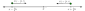
\includegraphics[width=.4\paperwidth]{deduction}
    \end{figure}

    \begin{definition}[Advection equation]
        \begin{equation*}
            u_{t}+du_{x}=0.
        \end{equation*}
    \end{definition}

    \begin{definition}[Diffusion equation]
        \begin{equation*}
            u_{t}=
            du_{xx}.
        \end{equation*}
    \end{definition}

    Let $h>0$, $h<<1$
\end{frame}

}

\nocite{*}
\printbibliography

\end{document}